\documentclass[10pt]{article}

\usepackage{amsmath}
\usepackage{CJK}
\usepackage{indentfirst}
\usepackage{fancyhdr}
\usepackage{graphicx}
\usepackage{longtable}
\usepackage{multirow}
\usepackage{listings}
\newcommand{\zcell}[2]{\begin{tabular}{@{}#1@{}}#2\end{tabular}}
\newcommand{\HRule}{\rule{\linewidth}{0.3mm}}

\begin{document}
\setlength{\parindent}{2em}
\begin{CJK}{UTF8}{gbsn}

\pagestyle{fancy}
\fancyhead{}
\lhead{XML文档编码与结构连接的研究与实现}
\rhead{\thepage}

\setlength{\topmargin}{3cm}
\begin{titlepage}
\begin{center}
{\huge \bfseries XML文档编码与结构连接\\研究与实现}\\
\HRule \\[0.4cm] 
\vspace{2cm}
\vspace{3cm}
{\large 计83{ }朱文雷{ }2008011369\\计85{ }任胜韦{ }2008011428}
\vfill
{\large 2010年12月28日}
\end{center}
\end{titlepage}
\setlength{\topmargin}{0cm}

\newpage
\tableofcontents
\newpage

\section{实验内容}
实现一个 xml 文件的关系查询。输入一个 xml 文件,要求将 xml 文件解析并且按照一定格式(格式自己定义)存储到 RDBMS 中,供用户查询各元素的连接关系。


\section{实现工具}
用 Microsoft SQL Server 2008 Express 作后端数据库,前端采用 Microsoft 的 Visual C\#, XML解析使用的是 C\# 中自带XML解析器 
XmlDocument. 用以下代码即可解析 XML :\\
\begin{verbatim}
XmlDocument xml_data = new XmlDocument();
xml_data.Load(xml_name);
\end{verbatim}

\section{XML编码}
XML 文档的编码我们采取的是普遍使用的区间编码,每一个结点的编码值由区间下界,区间上界和结点深度构成。XML 文档的编码工作是
由 Program.cs 中的 save 函数处理的。由区间编码的特点,用递归来实现区间编码会非常简单,而 save 函数就是一个
递归处理的过程,对整个 XML 实现区间编码。其伪代码如下:\\

\begin{lstlisting}[language=C,tabsize=4]
num = 0;
height = 0;

void save(XmlNode node){
	if(node == NULL)
		return;
    if(node has child){
        num ++;
		int temp = num;
		foreach(XmlNode child in node.ChildNodes){
			height ++;
			save(child);
			height --;
		}
		num ++;
		output(nodename, temp, num, height);
	}else{
		output(nodename, num+1, num+2, height);
		num += 2;
	}
}
\end{lstlisting}

\section{存储XML编码数据}
向 SQL Server 中导入数据我们采用速度较快的 \textbf{bulk insert} 将整个文件导入数据库实现。首先将前面的 XML 编码结果写入
文件 save.txt 中,然后采用 \textbf{bulk insert} 语句将整个文件数据导入。实际执行的数据库导入语句如下:\\

\begin{lstlisting}[language=sql]
bulk insert tree from 'save.txt' with 
    ( FIELDTERMINATOR=',',ROWTERMINATOR=';')
\end{lstlisting}

\section{数据库连接}
数据库连接使用 C\# 中提供的 SqlConnection 来实现,代码如下:\\
\begin{verbatim}
System.Data.SqlClient.SqlConnection mySqlconnection;
mySqlconnection = new SqlConnection(
                          "integrated security = SSPI;" + 
                          "DataBase =" + dbName + ";" + 
                          "Server = (local)\\SQLExpress");
mySqlconnection.Open();
\end{verbatim}

\section{实现结构连接}
\subsection{概述}
结构连接我们完全使用SQL查询实现,没有在取出数据后进行任何额外运算。这样做的优点是当数据量特别大时仍然能有不错的性能。
而如果把大量数据取出后再利用算法进行搜索的话,一方面没有充分利用数据库的能力,另一方面就会有数据量特别大时空间不够等问题。

结构连接在我们的代码中是由 Program.cs 中的 \textbf{search} 函数来实现的,给他不同的参数信息就能分别实现父子关系,祖先后代
关系查询。

\subsection{祖先后代关系查询}
祖先后代的查询方式如下: 首先将祖先和后代的所有结果查出来形成两个表,然后再在表中选择符合祖先后代关系的结点即可。由于我们
对 XML 采用的是区间编码,其祖先后代关系判断方法十分简单:\\

$$offspring \subset ancestor$$

写成数学表达式即 

$$offspring.low > ancestor.low \cap offspring.high < ancestor.high$$

故最后的 SQL 查询代码如下:\\
\begin{lstlisting}[language=sql,tabsize=2]
select * from 
	(select * from tableName where name='ancestor') as table1, 
	(select * from tableName where name='offspring') as table2 
	where (table1.low < table2.low) 
	and (table1.high > table2.high);
\end{lstlisting}

\subsection{父子关系查询}
有了祖先后代关系的查询之后,父子查询就变得简单了,只需要在上述条件中再加上一个 XML 高度相差1的条件即可.
其 SQL 查询代码如下:\\
\begin{lstlisting}[language=sql,tabsize=2]
select * from 
	(select * from tableName where name='father') as table1, 
	(select * from tableName where name='son') as table2 
	where (table1.low < table2.low) 
	and (table1.high > table2.high) 
	and (table1.height = table2.height-1);
\end{lstlisting}

\section{代码说明}
\begin{itemize}
\item Program.cs: 程序的入口部分,所有的逻辑部分也都由它负责。
\item Form1.cs: 界面部分,界面事件相应都写在这里。
\item Form1.Designer.cs 界面布局文件,由 Visual Studio 根据我们的设计自动生成。
\end{itemize}

\section{界面设计}
\subsection{启动界面}
下图是我们程序的初始界面。
\begin{center}
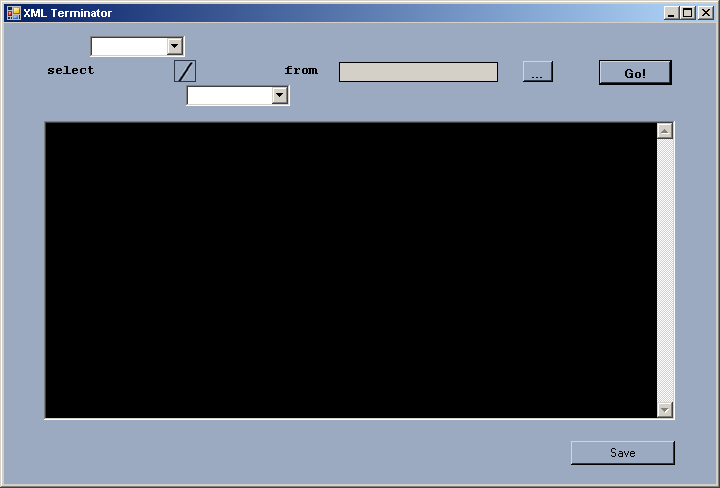
\includegraphics[width=0.9\linewidth]{startup.png}
\end{center}

界面右上角的按钮是 Go ,输入一个查询后点击Go按钮即可开始查询, Go 按钮左边的按钮
是 XML 文件选择按钮,点击它即可选择 XML 文件。左上方的两个方框是输入下拉选择框,既可以用户输入,也可以
通过下拉菜单选择相应的选项,两个框之间是查询类型转换按钮,初始时处于父子查询状态,点击它就可以在两种查询
之间转换。

界面中间的黑框是输出窗口,它会打印 log 输出和查询结果。输出窗口下面是保存按钮,可以将输出保存成文件。

\subsection{输出格式}
下图是我们的输出格式,每一个操作都会有输出提示和结果说明,最后会有总的执行时间统计输出。
\begin{center}
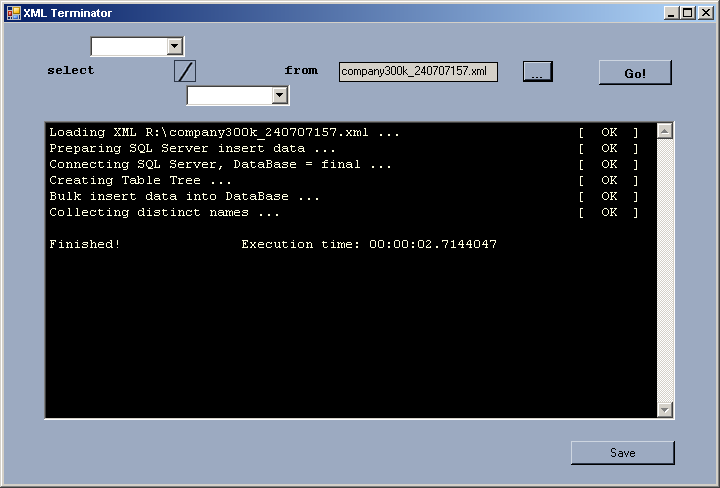
\includegraphics[width=0.9\linewidth]{loadxml.png}
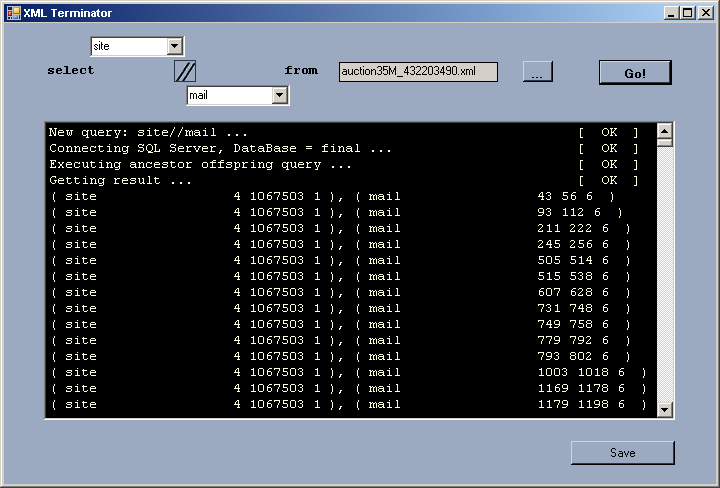
\includegraphics[width=0.9\linewidth]{test35_sitemail.png}
\end{center}

\subsection{结点选择}
如果直接输入不仅不方便而且还有可能出错,因此我们增加了结点选择功能,用下拉框的形式供用户选择 XML 中的结点。
\begin{center}
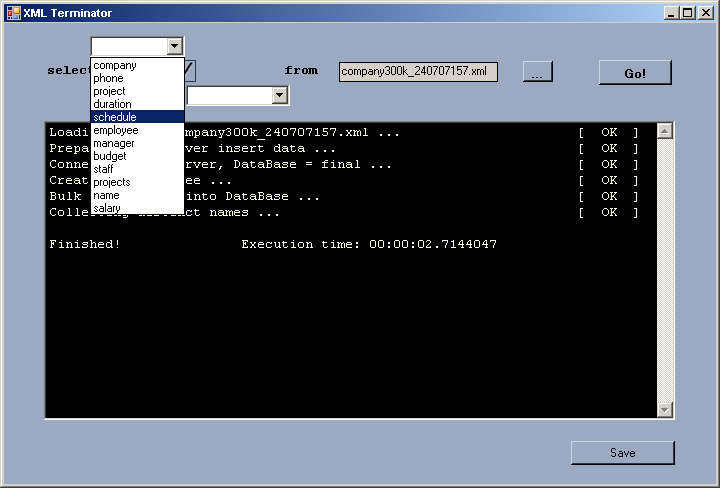
\includegraphics[width=0.9\linewidth]{selectnode.png}
\end{center}

\section{测试}
我们选择最大的测试文件 auction35M\_432203490.xml 来进行测试。

\subsection{XML解析}
如图,总时间需要 11 秒,包括了取出所有 XML 中不重复结点名字的操作(提供下拉选择框需要的数据),实际解析 XML 
加上插入数据库的时间在 8 秒以内。
\begin{center}
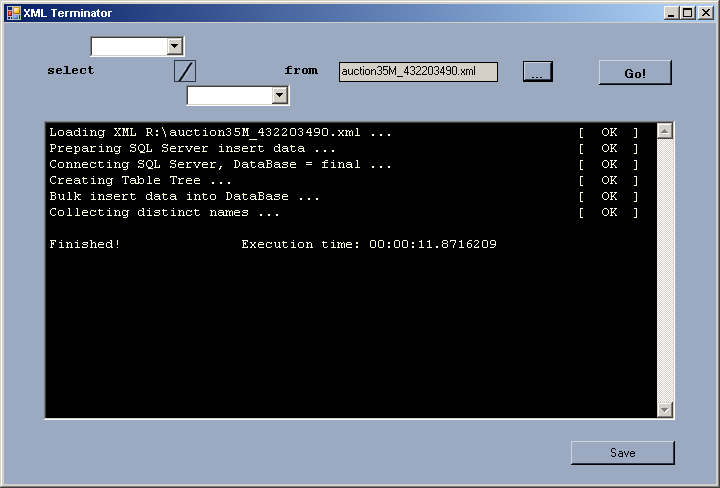
\includegraphics[width=0.9\linewidth]{load35.png}
\end{center}

\subsection{查询祖先后代关系}
我们查询 site//mail 作为测试,结果如下:\\
\begin{center}
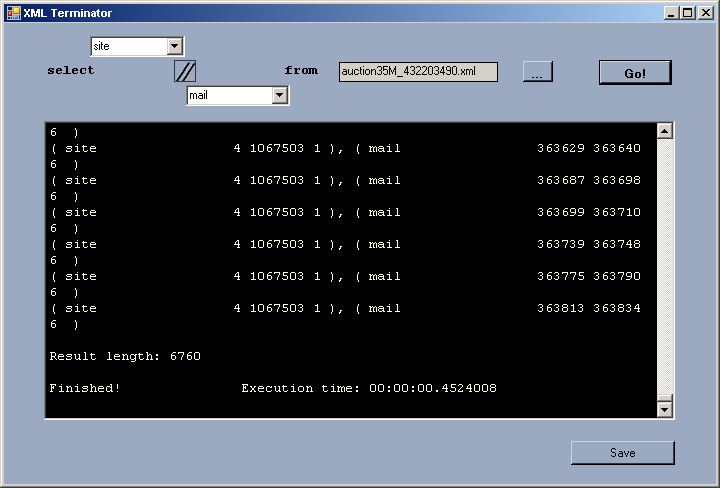
\includegraphics[width=0.9\linewidth]{test35_sitemail_time.png}
\end{center}
总时间为 0.45 秒,相当的快,最后结果有 6760 条。

\subsection{查询父子关系}
查询 mail//to 作为测试,结果如下:\\
\begin{center}
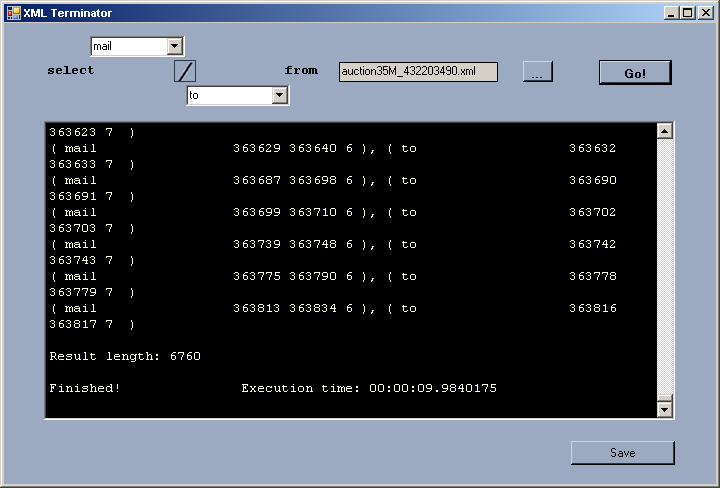
\includegraphics[width=0.9\linewidth]{test35_mailto_time.png}
\end{center}
由于 SQL 查询操作比查询多一个深度限制,时间稍长,总时间为 9.98 秒,最后结果有 6760 条。

\section{实验感想}
这次大实验总体来说还是比较简单的,只需要会使用数据库和了解 XML 的编码即可很好的完成,在实现的过程中遇到的问题也不多,
按照规范实现就直接得出了正确的结果。

但是这次实验还是让我们有很多收获,一方面,我们熟悉了数据库的使用,把课程中所学的关系代数和 SQL 的知识又巩固和加深了,
另一方面,我们接触了 XML 文件的结构和其编码,并把它的存储和数据库联系起来,解决了实际问题,这也让我们感觉到,这一学期的
数据库课让我们真正学到了东西,不仅仅有理论,还有实践。

\end{CJK}
\end{document}


